\section{Methodology: Global Namespace with Per-Subtree Consistency/Durability}
\label{sec:methodology-decoupled-namespaces}

In this section we describe CudeleFS, our file system that lets administrators
assign consistency and durability semantics to subtrees in the global
namespace. A \textbf{mechanism} is an abstraction and basic building block for
constructing consistency and durability guarantees. CudeleFS exposes these
mechanisms and the administrator composes them together to construct
\textbf{policies}. These policies are assigned to subtrees and they dictate how
the file system should handle operations within that subtree.  Below, we
describe the mechanisms, the policies, and the API for assigning policies to
subtrees.

\subsection{Cudele's Mechanisms}
\label{sec:cudeles-mechanisms}

% describe the figure
Figure~\ref{fig:decouple} shows the mechanisms (labeled arrows) in Cudele and
which daemon(s) they are performed by.  Table~\ref{table:mechanisms} has a
description of what each mechanism does.  Of the 6 mechanisms in
Figure~\ref{fig:decouple} only 4 had to implemented and just 1 required changes to
the underlying storage system itself.

\subsubsection{No Changes} ``RPCs" and ``Stream" are part of the default CephFS
implementation; they are used to get strong consistency and global durability,
respectively.  Using existing configuration settings in Ceph we can turn
``Stream" on and off.  If it is off, then the metadata servers will not save
journals in the object store and the daemons that apply the journal to the
metadata store will never run.

\subsubsection{Library} for ``Create", ``Nonvolatile Apply", ``Local/Global
Persist", CudeleFS provides a library for clients to link into and all
operations are performed by the client.  Decoupled clients use the ``Create"
mechanism to append metadata updates to a local, in-memory journal.  For
``Local Persist", clients write serialized log events to a file on local disk
and for ``Global Persist", clients push the journal into the objects store. The
overheads for both ``Local Persist" and ``Global Persist" is the write
bandwidth of the local disk and object store, respectively.  ``Nonvolatile
Apply" replays the client's journal onto the metadata cluster's metadata store.
The client's in-memory journal is written into the object store and the
metadata servers are restarted. When the metadata servers re-initialize, they
notice new journal updates in the object store and replay the events onto their
in-memory metadata stores.  These implementations required no changes to CephFS
because the metadata servers know how to read the events the library is writing
into the object store.  By re-using the journal subsystem to implement the
namespace decoupling, Cudele leverages the write/read optimized data
structures, the formats for persisting events (similar to TableFS's
SSTables~\cite{ren:atc2013-tablefs}), and the functions for replaying events
onto the internal namespace data structures.

\begin{figure}[tb]
\centering
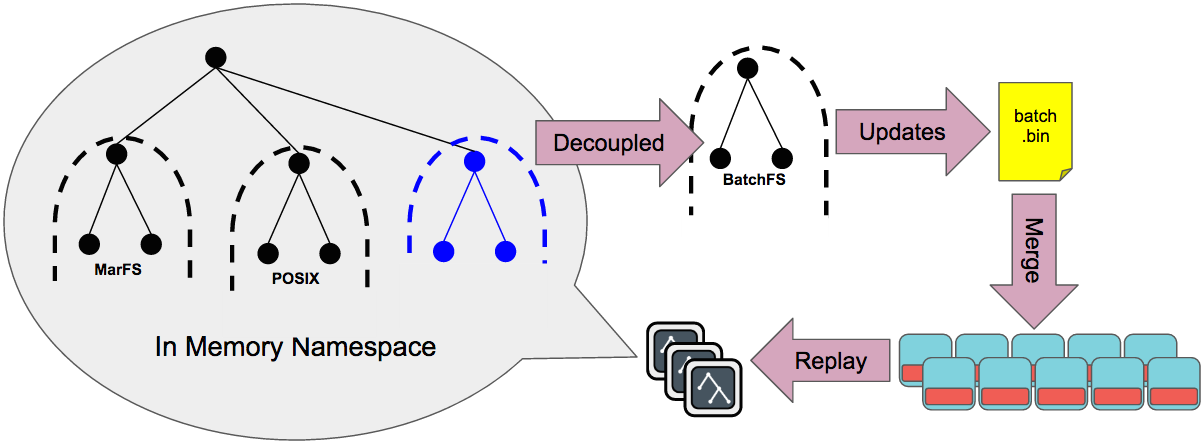
\includegraphics[width=90mm]{figures/fig-decouple.png}
\caption{Applications decouple the namespace, write updates to a local journal,
and delay metadata updates using the CudeleFS Mechanisms }\label{fig:decouple}
\end{figure}

% - how it makes no gaurantees
\subsubsection{Changes to Metadata Server} the ``Volatile Apply" mechanism
takes an in-memory journal on the client and applies the updates directly to
the in-memory namespace maintained by the metadata servers. We say volatile
because -- in exchange for peak performance -- Cudele makes no consistency or
durability guarantees while ``Volatile Apply" is executing.  If a concurrent
update from a client occurs there is no rule for resolving conflicts and if the
client or metadata server crashes there may be no way to recover.

% difference between apply and volatile apply
In contrast, ``Nonvolatile Apply" uses the the object store to apply the
journal of updates from the client onto the metadata servers' metadata store.
``Nonvolatile Apply" is safer but has a performance overhead because objects in
the metadata store need to be read from and written back to the object store.

%The metadata store and journal
%are different ways of representing the namespace.  Cudele presents 6
%mechanisms: RPCs, Stream, Create, Volatile Apply, Local Persist, and Global
%Persist. ``RPCs" does round trip remote procedure calls to establish
%consistency; it is the default implementation for complying with POSIX in
%CephFS. ``Stream" has the metadata servers stream a journal of metadata updates
%into the object store. ``Create" allows clients to append metadata events to an
%in-memory journal. ``Volatile apply" 
% ``Local Persist" takes the in-memory journal and writes it to the
%client's disk. ``Global Persist" saves the journal as a an object in the object
%store from the client.  Next, we discuss how these mechanisms can be composed
%to get different consistency and durability semantics. 

\subsection{Defining Policies in Cudele}
\label{sec:setting-policies-with-cudele}

% describe table
The spectrum of consistency and durability guarantees that administrators can
construct is shown in Table~\ref{table:spectrum}. The columns are the different
consistency semantics and the rows cover the spectrum of durability guarantees.
For consistency: ``invisible" means the system does not handle merging updates
into a global namespace and it is assumed that middleware or the application
manages consistency lazily; ``weak" merges updates at some time in the
future ({\it e.g.}, when the system has time, when number of updates reaches a
certain threshold, when the client is done writing, etc.); and updates in
``strong" consistency are seen immediately by all clients. For durability,
``none" means that updates are volatile and will be lost on a failure. Stronger
guarantees are made with ``local", which means updates will be retained if the
client node recovers, and ``global", where all updates are always recoverable.

% which system they represent and which are impossible
Existing, state-of-the-art systems in HPC can be represented by the cells in
Table~\ref{table:spectrum}.  POSIX-compliant systems like CephFS and IndexFS
have global consistency and durability; DeltaFS uses ``invisible" consistency
and ``local" durability and BatchFS uses ``weak" consistency and ``local"
durability.  To compose the mechanisms administrators inject which mechanisms
(described in Section~\S\ref{sec:cudeles-mechanisms}) to run and which to use
in parallel using a domain specific language. 

% what is impossible
Although we can achieve all permutations of the different guarantees in
Table~\ref{table:spectrum}, not all of them make sense. For example, it
makes little sense to do \texttt{creates+RPCs} since both mechanisms do the same
thing or \texttt{stream+save} since ``global" durability is stronger and has
more overhead than ``local" durability. 

% talk of eventual consistency
The consistency and durability properties in Table~\ref{table:spectrum} are not
guaranteed until all mechanisms in the cell are complete. The compositions
should be considered atomic and there are no guarantees while transitioning
between policies. For example, updates are not deemed globally consistent until
they are safely saved in the object store. If a failure occurs during ``global
persist" or if we inject a new policy that changes a subtree from ``local
persist" to ``global persist", CudeleFS no guarantee until the mechanisms are
complete.

\begin{table}
\begin{tabular}{ r | l }
  Mechanism         & Description \\\hline
  RPCs              & round trip remote procedure calls \\
  Stream            & stream journal into object store \\
  Create            & events appended to in-memory journal \\
  Volatile Apply    & apply to metadata store in obj store \\
  Nonvolatile Apply & apply to metadata store in memory \\
  Local Persist     & journal saved to client's disk \\
  Global Persist    & journal saved in object store \\
\end{tabular}
\caption{Cudele's mechanisms are composed together to form consistency and
durability semantics.\label{table:mechanisms}} 
\end{table}

\begin{table}[t]
\begin{center}
\caption{Future programmers can explore the consistency (C) and
durability (D) spectrums by composing Cudele mechanisms. 
\label{table:spectrum}}
\begin{tabular}{ l | l | l | l }
  C \(\rightarrow\) &&& \\  
  D \(\downarrow\)  	     & invisible         & weak        & strong  \\\hline
  none                       & create            & create          & RPCs    \\
                             &                   & +volatile apply &         \\\hdashline
  local                      & create            & create          & RPCs    \\
                             & +local persist    & +local persist  & +local  \\
                             &                   & +volatile apply &  persist\\\hdashline
  global                     & create            & create          & RPCs    \\
                             & +global persist   & +global persist & +stream \\
                             &                   & +volatile apply &         \\
\end{tabular}
\end{center}
\end{table}

\subsection{Cudele Namespace API}
\label{sec:cudele-namespace-api}

% the interface
The interface for setting the subtree policies is with \{path,
\(<\)block\(|\)overwrite\(>\), pre-allocated inodes\} tuples. For example:

\texttt{(msevilla/mydir, policies.yml)}

would decouple the path \texttt{msevilla/mydir} and would apply the policies in
\texttt{policies.yml}. The policies file supports the following values:

\begin{itemize}

  \item \texttt{allocated\_inodes}: the number of inodes to allocate to the
  decoupled namespace (default 100)

  \item \texttt{interfere\_callback}: how to handle a request from another
  client targeted at the now decoupled subtree (default \texttt{overwrite})

  \item \texttt{consistency\_callback}: which consistency model to use (default
  \texttt{RPCs})

  \item \texttt{durability\_callback}: which durability model to use (default
  \texttt{stream})

\end{itemize}

% description
For \texttt{block}, any requests to this part of the namespace returns with
``Device is busy", which will spare the metadata server from wasting resources
for updates that may get overwritten. If the application does not mind losing
updates, for example it wants approximations for results that take too long to
compute, it can select \texttt{overwrite}. In this case, metadata will be
written and the computation from the decoupled namespace will take priority at
merge time because the results are more accurate.

% examples
Given these default values decoupling the namespace with an empty policies file
would give the application 100 inodes but the subtree would behave like the
existing CephFS implementation. To implement DeltaFS on CudeleFS, the user
would use the configuration from Listing~\ref{src:deltafs}. BatchFS's merging
back into the global namespace can be achieved with the configuration in
Listing~\ref{src:batchfs}.

%\begin{listing}
%\begin{minted}[frame=single,
%               framesep=3mm,
%               xleftmargin=21pt,
%               tabsize=4]{js}
%{     
%    "allocated_inodes": "-"
%    "interfere_policy": "-"
%    "consistency": "RPCs"
%    "durability": "stream"
%}
%\end{minted}
%\caption{Existing CephFS on Cudele.}
%\label{src:batchfs}
%\end{listing}
